% !TEX root =  ../main_iclr.tex

%\subsection{Data and preprocessing}

To evaluate our model, we use a collection of chemical reactions extracted from the US patent database \citep{Lowe2017}.
We take as our starting point the 479,035 reactions, along with the training, validation, and testing splits 
which were used by \citet{jin2017predicting}, referred to as the USPTO dataset.
This data consists of a list of reactions. Each reaction is a reaction SMILES string \citep{weininger1988smiles} and a list of bond changes.
SMILES is a text format for molecules that lists the molecule as a sequence of atoms and bonds.
The bond change list tells us which pairs of atoms have different bonds in the the reactants versus the products (note that this can be directly determined from the SMILES string).
Below, we describe two data processing techniques that allow us to identify reagents, reactions with LEF topology, and extract an underlying electron path. Each of these steps can be easily implemented with the open-source chemo-informatics software RDKit \citep{rdkit}.

%Before we can apply our method, we perform two data preprocessing tasks described  below (using the open-source chemo-informatics software RDKit \citep{rdkit}). 
%These steps automatically extract a subset of data appropriate for training our of electron movement during a reaction.
 
\paragraph{Reactant and Reagent Seperation}
Typically, reaction SMILES strings are split into three parts --- reactants, reagents, and products.
The reactant molecules are those which are consumed during the course of the chemical reaction to form the product, 
while the {\em reagents} are any additional molecules which provide context under which the reaction occurs (for example, catalysts),
but do not explicitly take part in the reaction itself; an example of a reagent is shown in Figure~\ref{fig:task-overview}.


Unfortunately, the USPTO dataset as extracted does not differentiate between reagents and reactants.
We elect to preprocess the entire USPTO dataset by separating out the reagents from the reactants using the process outlined in \citet{schwaller2017found}, where we classify as a reagent any molecule for which either 
(i) none of its constituent atoms appear in the product, or 
(ii) the molecule appears in the product SMILES completely unchanged from the pre-reaction SMILES.
This allows us to properly model molecules which are included in the dataset but do not materially contribute to the reaction.

\paragraph{Identifying reactions with linear electron topology}
To train our model, we need to (i) identify reactions in the USPTO dataset with LEF topology, and (ii) have access to an electron path for each reaction. 
% from the SMILES strings and bond changes.
%Furthermore, not every reaction in the USPTO dataset has a linear electron topology; 
%such reactions (for example, multi-step reactions and cycloadditions) will not have a single unique path through the atoms 
%which describes the movement of the electrons. 
Figure \ref{fig:dataset_steps} shows the steps necessary to identify and extract the electron paths from reactions exhibiting LEF topology. We provide further details in Appendix \ref{sect:electron_path_identify}.


\begin{figure*}
\centering
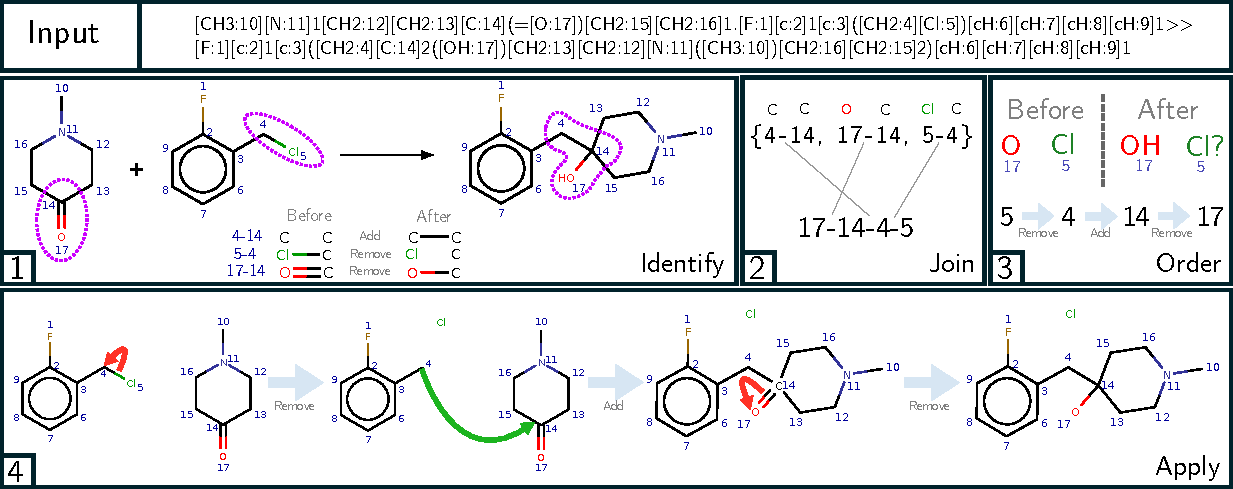
\includegraphics[width=1.\textwidth]{imgs/dataset_steps}
\caption{
Example of how we turn SMILES reaction string into an ordered electron path, for which we can train \ourModel on. 
This consists of a series of steps: 
(1) Identify bonds that change by comparing bond triples (source node, end node, bond type) between the reactants and products. 
(2) Line up the bond changes so that one of the atoms in consecutive bond changes overlap (for reactions which do not have linear electron flow topology, such as multi-step reactions, this will not be possible and so we discard these reactions).
(3) Work out the direction of the path. A gain of charge (or analogously the gain of hydrogen as H$^+$ ions without changing charge, such as in the example shown) indicates that the electrons have arrived at this atom; and vice-versa for the start of the path.
When details about both ends of the path are missing from the SMILES string we fall back to using an element's {\em electronegativity} to estimate the direction of our path, with more electronegative atoms attracting electrons towards them and so being at the end of the path. 
(4) The extracted electron path deterministically determines a series of intermediate molecules which can be used for training \ourModel. 
Paths that do not consist of alternative add and removal steps and do not result in the final recorded product do not exhibit LEF topology and so can be discarded.
}
\label{fig:dataset_steps}
\end{figure*}

Applying these steps, we discover that $73\%$ of the USPTO dataset consists of LEF reactions (349,898 total reactions, of which 29,360 form the held-out test set).

% give us 349,898 total 
% The end result of this is extracted reaction paths for those entries in the USPTO dataset which 
% correspond to reactions of linear topology.
% This comprises $73\%$ of the dataset, containing 349,898 total reactions, of which 29,360 form the held-out test set.






